\documentclass[11pt,a4paper]{article}

\usepackage[utf8]{inputenc}
\usepackage[T1]{fontenc}
\usepackage[brazil]{babel}
\usepackage[margin=2.5cm]{geometry}
\usepackage{amsmath,amssymb}
\usepackage{enumitem}
\usepackage{graphicx}
\usepackage{float}
\usepackage[hidelinks]{hyperref}

\graphicspath{{figures/}}
\setlength{\parskip}{0.4em}

\begin{document}

\section{A pergunta}

Detectores de \emph{deepfake} de áudio de ponta costumam ser treinados em inglês.
Queremos entender quais pistas acústicas um detector usa para decidir se um áudio
é real ou falso, e como essas pistas mudam quando o modelo é levemente adaptado ao
português brasileiro. Em resumo, duas perguntas:

\begin{enumerate}[label=\textbf{Q\arabic*.}]
  \item As pistas mudam entre um modelo \emph{zero-shot} e um adaptado?
  \item Se mudam, o que muda (para onde o foco vai no espectro, e se isso se
        relaciona com os erros do modelo)?
\end{enumerate}

O interesse é populacional: descrever o comportamento do detector sobre um
conjunto representativo de áudios, de forma estatística e verificável.

\section{O plano em uma página}

Vamos comparar dois detectores sobre o mesmo codificador de fala congelado
(wav2vec~2.0 / XLS-R), o que isola o efeito da adaptação:

\begin{itemize}[nosep]
  \item $D_{\mathrm{zs}}$: o head de decisão original, sem ajuste;
  \item $D_{\mathrm{ad}}$: um head leve (regressão logística) treinado sobre os
        \emph{embeddings} em português.
\end{itemize}

Sobre esse par, faremos duas análises complementares, ambas na mesma partição de
frequência (bandas em escala mel):

\begin{itemize}[nosep]
  \item \textbf{associativa}, que mede quais bandas acompanham o score;
  \item \textbf{causal}, que mede quais bandas, ao serem removidas do áudio, de
        fato alteram o score.
\end{itemize}

Em seguida, mediremos a convergência entre as duas e faremos uma etapa
confirmatória ligada aos erros do detector.

\section{Dados}

Usaremos o corpus BRSpeech-DF (cerca de 459 mil clipes, muito desbalanceado, com
mais falsos que reais). Como o objetivo é explicabilidade, e não \emph{ranking},
montaremos um conjunto equilibrado de análise: todo o áudio real disponível no
teste (1.320 clipes, a classe escassa) somado a 1.500 falsos, num total de 2.820
clipes, sem sobreposição com o treino do head.

\section{O que faremos, etapa a etapa}

\begin{description}[leftmargin=1.4em]
  \item[Pré-processamento.] Mono, 16~kHz, janela de cerca de 4 segundos e
        normalização. As \emph{features} são extraídas do mesmo sinal que entra no
        detector, não do áudio bruto.
  \item[Descrição acústica.] Energia log-mel por banda, resumida por média e
        desvio ao longo do tempo. Escolhemos essa descrição por ser localizada em
        frequência, o que permite comparar as duas análises banda a banda.
  \item[Desempenho.] A métrica principal será a EER (o ponto em que as duas taxas
        de erro se igualam, quanto menor melhor), acompanhada de MCC e acurácia.
        Só analisaremos as pistas se a adaptação de fato melhorar a detecção.
  \item[Análise associativa.] Correlação de Spearman entre cada banda e o score,
        calculada dentro de cada classe para evitar correlação espúria, com
        correção estatística para múltiplos testes. O sinal indica o sentido:
        positivo quando mais energia na banda acompanha um score mais alto de
        \emph{spoof}; negativo quando acompanha um score mais baixo (na direção de
        \emph{bonafide}).
  \item[Análise causal.] Remoção de uma banda por vez (filtro de fase zero) e
        medição da queda no score, com intervalos de confiança por \emph{bootstrap}.
  \item[Convergência.] Comparação, banda a banda, entre o perfil causal e o
        associativo. Como haverá poucas bandas, será uma indicação descritiva, não
        um teste com poder.
  \item[Confirmatória.] Testes estatísticos formais apenas nas pistas mais
        relevantes, ligados aos quadrantes de acerto e erro, com controle de
        falsas descobertas. Esta é a única parte inferencial do estudo.
\end{description}

\section{Hipóteses}

\begin{itemize}[nosep]
  \item \textbf{H1 (descritiva).} As pistas de áudio que acompanham a decisão do
        detector não são as mesmas antes e depois da adaptação.
  \item \textbf{H2 (causal).} Ao remover uma faixa de frequência do áudio, as
        faixas que de fato mudam a decisão são diferentes nos dois modelos.
  \item \textbf{H3 (inferencial).} As pistas mais importantes se comportam de
        forma diferente quando o detector acerta e quando erra.
\end{itemize}

\section{O que o estudo vai entregar}

Uma comparação de desempenho entre os detectores, um perfil associativo e um
perfil causal por banda, uma medida de convergência entre eles e um conjunto de
testes confirmatórios. Juntas, essas saídas devem responder às duas perguntas de
forma verificável, com a evidência causal (a oclusão) como parte mais forte, por
ser a única baseada em intervenção direta no áudio.

\section{Achados preliminares}

As figuras a seguir vêm de uma primeira execução completa do pipeline. Elas
ilustram, na prática, cada pergunta e hipótese. Os valores são de um run inicial e
podem ser refinados.

\subsection*{Desempenho: a adaptação melhora a detecção}

Cada painel da Figura~\ref{fig:eer} traz duas curvas de erro que se movem em
direções opostas conforme ajustamos o limiar de decisão: a de rejeitar áudio real
(laranja) e a de deixar passar \emph{deepfake} (azul). O ponto em que elas se
cruzam é o EER, que resume o detector num único número. O modelo adaptado (painel
de baixo) cruza mais embaixo, ou seja, erra menos dos dois lados ao mesmo tempo: o
EER cai de 25,8\% para 20,9\% (com ganhos correspondentes em MCC e acurácia). Esse
resultado é a pré-condição do estudo, pois só faz sentido investigar as pistas de
um detector que de fato melhorou. O eixo horizontal está em escala \emph{logit}
porque as probabilidades se concentram perto de~1.

\begin{figure}[H]
  \centering
  \includegraphics[width=0.58\textwidth]{eer_threshold_zs_vs_ad}
  \caption{Taxas de erro em função do limiar (topo: \emph{zero-shot}; base:
  adaptado). O ponto preto marca o EER, onde as duas taxas se igualam.}
  \label{fig:eer}
\end{figure}

\subsection*{H1: as pistas associadas à decisão se deslocam}

Na Figura~\ref{fig:h1}, cada barra mede a associação entre a energia de uma faixa
de frequência e a decisão do detector (correlação de Spearman, calculada dentro de
cada classe). O sentido está na direção da barra: para cima quando mais energia
naquela faixa acompanha um score mais alto de \emph{spoof} (\(\rho>0\)) e para
baixo quando acompanha um score mais baixo, rumo a \emph{bonafide} (\(\rho<0\)). A
altura indica a intensidade da associação.

A figura tem dois painéis: o de cima usa a energia \emph{média} de cada faixa
(\(\mu\)) e o de baixo usa a \emph{variabilidade} dessa energia ao longo do tempo
(o desvio-padrão \(\sigma\), que é a dispersão, não exatamente a variância).

No painel da média (\(\mu\)), o \emph{zero-shot} mantém barras para cima em quase
todas as faixas (mais energia associada a \emph{spoof}), com destaque nos graves.
No adaptado, o sentido se inverte nas faixas médias (cerca de 1,1 a 3,9~kHz), onde
as barras apontam para baixo (mais energia associada a \emph{bonafide}).

No painel da variabilidade (\(\sigma\)), o sentido também se inverte entre os
detectores: no \emph{zero-shot} as barras apontam para baixo em quase todas as
faixas (energia mais oscilante associada a \emph{bonafide}), enquanto no adaptado
apontam para cima nas faixas médias e agudas (energia mais oscilante associada a
\emph{spoof}).

Em conjunto, é a leitura descritiva de H1: parecem mudar tanto a faixa que importa
quanto o sentido da associação (para \emph{spoof} ou para \emph{bonafide}) e o tipo
de pista (nível médio ou variabilidade).

\begin{figure}[H]
  \centering
  \includegraphics[width=\textwidth]{association_profile_signed_zs_vs_ad}
  \caption{Associação (Spearman com sinal) por faixa de frequência, em dois painéis:
  energia média (\(\mu\), acima) e variabilidade ao longo do tempo (\(\sigma\),
  abaixo). A direção da barra indica o sentido: para cima rumo a \emph{spoof}
  (\(\rho>0\)) e para baixo rumo a \emph{bonafide} (\(\rho<0\)); a altura, a
  intensidade. As faixas sombreadas são aquelas em que os dois detectores têm
  \emph{sinais opostos}, ou seja, onde a associação inverte de sentido entre o
  \emph{zero-shot} e o adaptado. Registro descritivo (H1).}
  \label{fig:h1}
\end{figure}

\subsection*{H2: as faixas que realmente decidem mudam}

Aqui intervimos no áudio: removemos uma faixa de frequência por vez e medimos
quanto a probabilidade de \emph{spoof} cai (Figura~\ref{fig:h2}). Barras positivas
indicam faixas que sustentam a decisão de \emph{falso}; barras negativas, faixas
que empurram para \emph{real}. A região sombreada é o intervalo de confiança. O
\emph{zero-shot} usa quase todo o espectro (efeito espalhado), enquanto o adaptado
é mais seletivo e chega a usar uma faixa média como indício de áudio real (a barra
que inverte o sinal). É a evidência causal de H2.

\begin{figure}[H]
  \centering
  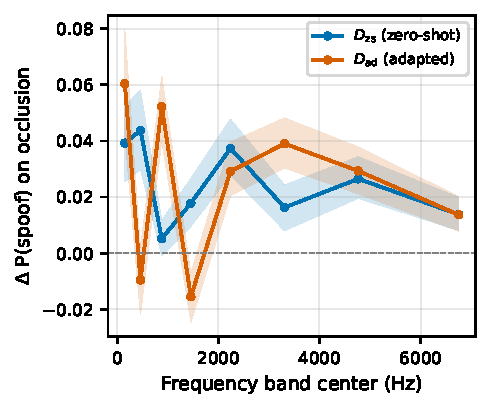
\includegraphics[width=0.5\textwidth]{occlusion_overlay_zs_vs_ad}
  \caption{Queda média da probabilidade de \emph{spoof} ao ocluir cada faixa, com
  intervalo de confiança de 95\%. Registro causal (H2).}
  \label{fig:h2}
\end{figure}

\subsection*{As duas análises concordam?}

A Figura~\ref{fig:conv} compara, na mesma grade de faixas, as duas visões, um
painel por detector. As barras (eixo à esquerda) são o efeito \emph{causal}, quanto
a probabilidade de \emph{spoof} muda ao silenciar a faixa (\(|\Delta P|\)); a linha
(eixo à direita) é a \emph{associação} da faixa com a decisão (\(|\rho|\), como na
Figura~\ref{fig:h1}). O \emph{agreement} \(\rho\) no título mede se os dois perfis
têm o mesmo formato ao longo das faixas (Spearman, entre \(-1\) e \(1\): perto de
\(1\) sobem e descem juntos; perto de \(0\), pouca relação; perto de \(-1\), formato
oposto).

Com cautela (só 8 faixas, leitura descritiva): no \emph{zero-shot} as duas visões
tendem a concordar, ambas mais fortes nos graves (\(\rho=0{,}69\), marginal); no
adaptado elas se descolam (\(\rho=0{,}10\)), com o efeito causal nos graves e a
associação nos médios. Nenhum é significativo a 5\%.

\begin{figure}[H]
  \centering
  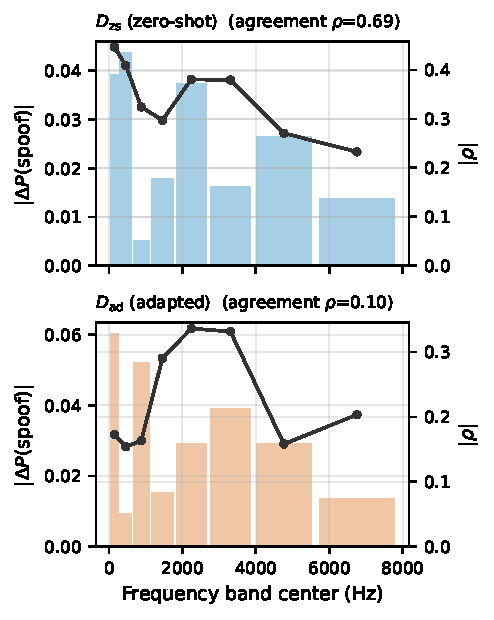
\includegraphics[width=0.5\textwidth]{spine_convergence_zs_vs_ad}
  \caption{Convergência entre os perfis causal e associativo na mesma grade de
  faixas (um painel por detector). Barras (eixo esquerdo): efeito causal da
  oclusão, \(|\Delta P(\mathrm{spoof})|\). Linha (eixo direito): força da
  associação com a decisão, \(|\rho|\) de Spearman. O \emph{agreement} \(\rho\) no
  título é a correlação entre as barras e a linha ao longo das faixas.}
  \label{fig:conv}
\end{figure}

\subsection*{H3: as pistas se ligam aos erros}

Por fim, ligamos as pistas mais relevantes aos erros do detector
(Figura~\ref{fig:h3}). A figura responde a duas perguntas, uma por painel, sempre
com uma faixa de frequência por linha. Cada ponto é o \emph{tamanho do efeito}; a
barrinha horizontal é o intervalo de confiança e a linha tracejada marca o
``sem diferença''. Ponto cheio significa diferença estatisticamente confiável
(pós-correção de falsas descobertas); ponto vazio, não.

\emph{Painel da esquerda --- a energia média muda quando um áudio real é
rejeitado por engano?} A maioria dos pontos cai dentro da faixa cinza de
``efeito pequeno'': as médias mal mudam entre real aceito e real rejeitado (TN vs
FP). Alguns são significativos apenas por causa do $N$ grande, mas o efeito
prático é modesto.

\emph{Painel da direita --- a variabilidade muda quando um \emph{spoof} passa
despercebido?} Aqui está o sinal mais forte: nas faixas graves, os pontos ficam
bem à direita do zero, ou seja, os \emph{spoofs} que o detector \emph{captura}
oscilam mais que os que \emph{passam} (os que escapam são mais ``lisos'', com
energia mais estável). É a evidência inferencial de H3.

\begin{figure}[H]
  \centering
  \includegraphics[width=0.95\textwidth]{confirmatory_effects_ad}
  \caption{Pistas ligadas aos erros (modelo adaptado). Uma faixa de frequência
  por linha. \emph{Esquerda}: diferença de \emph{média} entre real aceito e real
  rejeitado por engano (TN vs FP), em Cohen's $d$; a faixa cinza marca ``efeito
  pequeno''. \emph{Direita}: diferença de \emph{variabilidade} entre \emph{spoof}
  detectado e \emph{spoof} que passou (TP vs FN), em $\log_2$ da razão de desvios;
  valores positivos indicam mais variabilidade nos \emph{spoofs} detectados. Ponto
  cheio: significativo ($q<0{,}05$); vazio: não. Linha tracejada: sem diferença.}
  \label{fig:h3}
\end{figure}

\end{document}
